\documentclass[12pt]{article}
\usepackage{amsmath}
\usepackage{amsfonts}   % if you want the fonts
\usepackage{amssymb}    % if you want extra symbols
\usepackage{graphicx}   % need for figures
\usepackage{xcolor}
\usepackage{bm}
\usepackage{secdot}		
\usepackage{mathptmx}
\usepackage{float}
\usepackage[utf8]{inputenc}
\usepackage{textcomp}
\usepackage[hang,flushmargin,bottom]{footmisc} % footnote format

\usepackage{titlesec}
\titleformat{\section}{\normalsize\bfseries}{\thesection.}{1em}{}	% required for heading numbering style
\titleformat*{\subsection}{\normalsize\bfseries}

\usepackage{tocloft}	% change typeset, titles, and format list of appendices/figures/tables
\renewcommand{\cftdot}{}	
\renewcommand{\contentsname}{Table of Contents}
\renewcommand{\cftpartleader}{\cftdotfill{\cftdotsep}} % for parts
\renewcommand{\cftsecleader}{\cftdotfill{\cftdotsep}}
\renewcommand\cftbeforesecskip{\setlength{4pt}{}}
\addtolength{\cftfignumwidth}{1em}
\renewcommand{\cftfigpresnum}{\figurename\ }
\addtolength{\cfttabnumwidth}{1em}
\setlength{\tabcolsep}{35pt}

\usepackage{enumitem}         % to control spacing between bullets/numbered lists

\usepackage[hidelinks]{hyperref}
\hypersetup{
	colorlinks = true,
urlcolor ={blue},
citecolor = {.},
linkcolor = {.},
anchorcolor = {.},
filecolor = {.},
menucolor = {.},
runcolor = {.}
pdftitle={},
pdfsubject={},
pdfauthor={},
pdfkeywords={}
}
\urlstyle{same}

\usepackage{epstopdf} % converting EPS figure files to PDF

\usepackage{fancyhdr, lastpage}	% formatting document, calculating number of pages, formatting headers
\setlength{\topmargin}{-0.5in}
\setlength{\headheight}{40pt}
\setlength{\oddsidemargin}{0.25in}
\setlength{\evensidemargin}{0.25in}
\setlength{\textwidth}{6.0in}
\setlength{\textheight}{8.5in}

\usepackage{caption} % required for Figure labels
\captionsetup{font=small,labelfont=bf,figurename=Fig.,labelsep=period,justification=raggedright} 

\renewcommand\contentsname{Indice}


%   	BEGIN DOCUMENT 
%%%%%%%%%%%%%%%%%%%%%%%%%%%%%%%%%%%%%%%%%%%%%%%%%%%%%%%%%%%%%%%%%%%%
\begin{document}
	\urlstyle{rm} % Format style of \url   
%%%%%%%%%%%%%%%%%%%%%%%%%%%%%%%%%%%%%%%%%%%%%%%%%%%%%%%%%%%%%%%%%%%%
\begin{figure}[h!]
\vskip1in
\begin{center}

\includegraphics[scale = 2]{fig/logo.jpg}
\end{center}
\end{figure}

\begin{center}
\large{\textbf{PoS Tagger per lingue morte}}
\end{center}

\vskip2.5cm

\begin{center}
a cura di
\end{center}

\vskip0.6cm

\begin{center}
\textbf{Pier Felice Balestrucci}\\
\textbf{Miriam Fasciana}\\
\end{center}

\vskip3.5cm
 
\begin{center}
\textbf{Relazione del progetto di TECNOLOGIE DEL LINGUAGGIO NATURALE}
\end{center}

\begin{center}
\textbf{Università degli studi di Torino 2020/2021}
\end{center}
%%%%%%%%%%%%%%%%%%%%%%%%%%%%%%%%%%%%%%%%%%%%%%%%%%%%%%%%%%%%%%%%%%%%
%   Table of Contentsì
%%%%%%%%%%%%%%%%%%%%%%%%%%%%%%%%%%%%%%%%%%%%%%%%%%%%%%%%%%%%%%%%%%%%
\newpage
\begin{center}
\tableofcontents
\end{center}
\pagebreak
%%%%%%%%%%%%%%%%%%%%%%%%%%%%%%%%%%%%%%%%%%%%%%%%%%%%%%%%%%%%%%%%%%%%
\section{Introduzione}
L’esercizio proposto per la prima parte d’esame è l’implementazione di un PoS tagger statistico basato su HMM per il greco antico e per il latino. Nel dettaglio, si è implementata la fase di learning e decoding con l’algoritmo di Viterbi e si è valutato il sistema applicando diverse strategie di smoothing. Infine, i risultati sono stati confrontati rispetto ad una baseline.
\\Il progetto è consultabile all'indirizzo Github: \href{https://github.com/TLN2021/PosTagger}{TLN2021/PosTagger}.
%%%%%%%%%%%%%%%%%%%%%%%%%%%%%%%%%%%%%%%%%%%%%%%%%%%%%%%%%%%%%%%%%%%%
\section{Fase di learning}
Come prima cosa è stata implementata la fase di learning in cui si sono calcolate le probabilità di transizione e quelle di emissione.
\\Per svolgere questa e le successive fasi è stato necessario ricercare i possibili PoS tag presenti nei Treebank del greco e del latino del progetto UD. 
\\Di seguito è mostrato il risultato della ricerca.

\begin{figure}[!h]
   \centering
   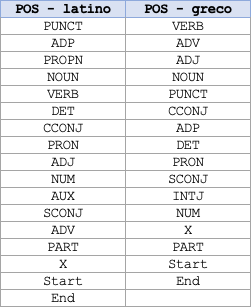
\includegraphics[scale=0.5]{fig/POSLatinoGreco.png}
   \caption{Tag per il latino e il greco}\label{fig:pos}
\end{figure}

Successivamente sono state calcolate le probabilità di transizione e di emissione sulla base della modellazione formale del problema del PoS tagging.
\\Più in particolare, le probabilità di transizione sono state calcolate dividendo la frequenza all’interno del corpus del tag $t_i$ preceduto dal tag $t_{i-1}$, per il numero di volte in cui compare il tag $t_{i-1}$.

\[ P(t_1^n) \approx \prod_{n=1}^n P(t_i|t_{1-1})\]


Queste sono state memorizzate in una \textit{matrice} di dimensione $pos * pos$ in cui ogni cella indica il numero di volte in cui il tag in una determinata colonna precede quello nella riga.

Le probabilità di emissione sono state calcolate dividendo il numero di volte con cui è assegnato un certo tag al termine per il numero di volte in cui quello stesso tag compare in tutto il corpus.

\[ P(w_{1}^n|t_1^n) \approx \prod_{i=1} P(w_i|t_i)\]

In questo caso si è optato per un \textit{dizionario} per memorizzare le probabilità dove le chiavi sono le parole del corpus e i valori di queste sono le probabilità per cui una parola essere etichettata con un tag.
%%%%%%%%%%%%%%%%%%%%%%%%%%%%%%%%%%%%%%%%%%%%%%%%%%%%%%%%%%%%%%%%%%%%
\section{Fase di decoding}
Nella fase di decoding si è implementato l’algoritmo di Viterbi. Si precisa che, affinché i dati non fossero affetti da errori di approssimazione essendo le probabilità molto piccole, i calcoli sono stati effettuati convertendoli in forma logaritmica.
\\
L’algoritmo è suddiviso in quattro parti:
\begin{enumerate}
    \item \textbf{fase di inizializzazione}: nella matrice di Viterbi viene inserita la probabilità che un certo stato sia il primo PoS della sequenza
    \item \textbf{fase ricorsiva}: per tutte le parole dalla seconda all’ultima viene calcolato il valore di viterbi utilizzando la formula $v_{t}(j) = max_{i=1,..,n}v_{t}(j)*a_{ij}*b_{j}(o_{t})$  dove:
    \begin{itemize}
        \item $v_{t}(j)$ = valore di viterbi per la parola t ed il pos j
        \item $a_{ij}$ = probabilità di transizione dallo stato i allo stato j
        \item $b_{j}(o_{t})$ = probabilità di emissione per la parola t ed il pos j
    \end{itemize}
    \item \textbf{fase di terminazione}: si calcola la probabilità per cui un certo tag sia quello finale
    \item \textbf{ultima fase}: utilizza il vettore dei backpointer per risalire al giusto percorso di stati che porta dallo stato finale a quello iniziale della matrice di Viterbi.
\end{enumerate} 

\begin{figure}[H]
   \centering
   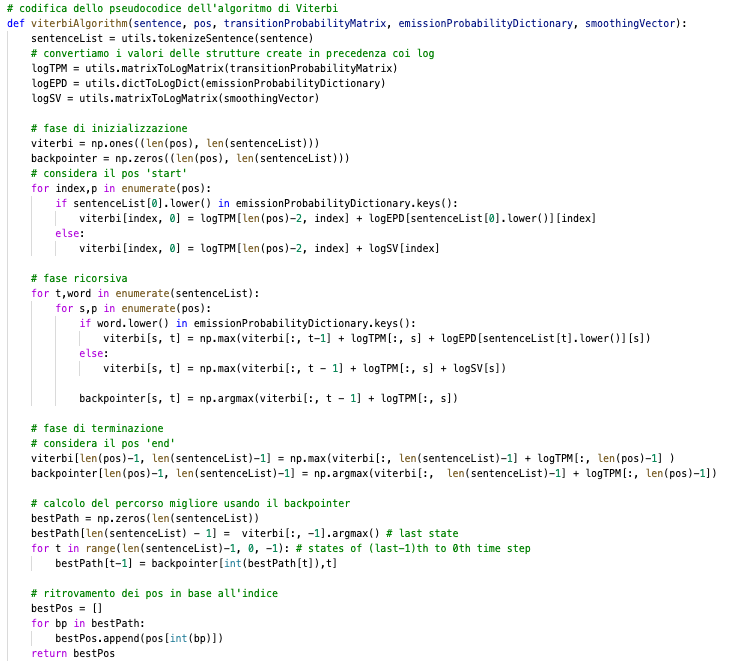
\includegraphics[scale=0.5]{fig/ViterbiCodice.png}
   \caption{Codice algoritmo di Viterbi}\label{fig:Viterbi}
\end{figure}
%%%%%%%%%%%%%%%%%%%%%%%%%%%%%%%%%%%%%%%%%%%%%%%%%%%%%%%%%%%%%%%%%%%%
\section{Strategie di smoothing}
Come si vede dalla figura \ref{fig:Viterbi}, lo smoothing permette di gestire casi in cui il sistema deve affrontare termini sconosciuti. 
\\Gli approcci adottati sono diversi:
\begin{itemize}
    \item la prima strategia è assumere che tutte le parole sconosciute siano dei nomi;
    \item un secondo modo, invece, è quello di assumere che queste siano o nomi o verbi;
    \item è possibile distribuire una probabilità omogenea a tutti i PoS;
    \item un’altra tecnica molto ingegnosa è quella di allenare il sistema su un secondo corpus - in questo caso il development set del progetto UD - calcolando le probabilità che parole sconosciute possano essere etichettate con un certo PoS;
    \item l’ultimo approccio implementato è basato sulla sintassi: si controlla che un termine abbia un certo suffisso o prefisso per dedurre che questo possa essere classificato in un certo modo.
\end{itemize} 

Di seguito sono riportate le feature sintattiche - suffissi - usate per la classificazione:
\begin{figure}[H]
   \centering
   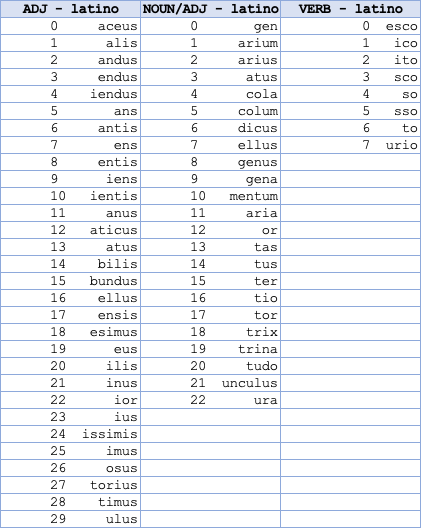
\includegraphics[scale=0.5]{fig/SintassiLatino.png}
   \caption{Feature sintattiche per il latino}\label{fig:sntxLatino}
\end{figure}

\begin{figure}[H]
   \centering
   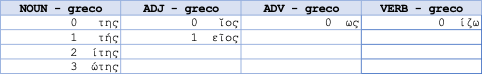
\includegraphics[scale=0.5]{fig/SintassiGreco.png}
   \caption{Feature sintattiche per il greco}\label{fig:sntxGreco}
\end{figure}

\textbf{Nota}: gli accorgimenti sintattici ritrovati per il greco sono inferiori a quelli latini per motivi di ritrovamento. Seppur in numero basso essi hanno portato come si vedrà comunque a miglioramenti.
%%%%%%%%%%%%%%%%%%%%%%%%%%%%%%%%%%%%%%%%%%%%%%%%%%%%%%%%%%%%%%%%%%%%
\section{Valutazione}
Nella seguente sezione si mostrano i risultati ottenuti dal sistema.

\begin{figure}[H]
   \centering
   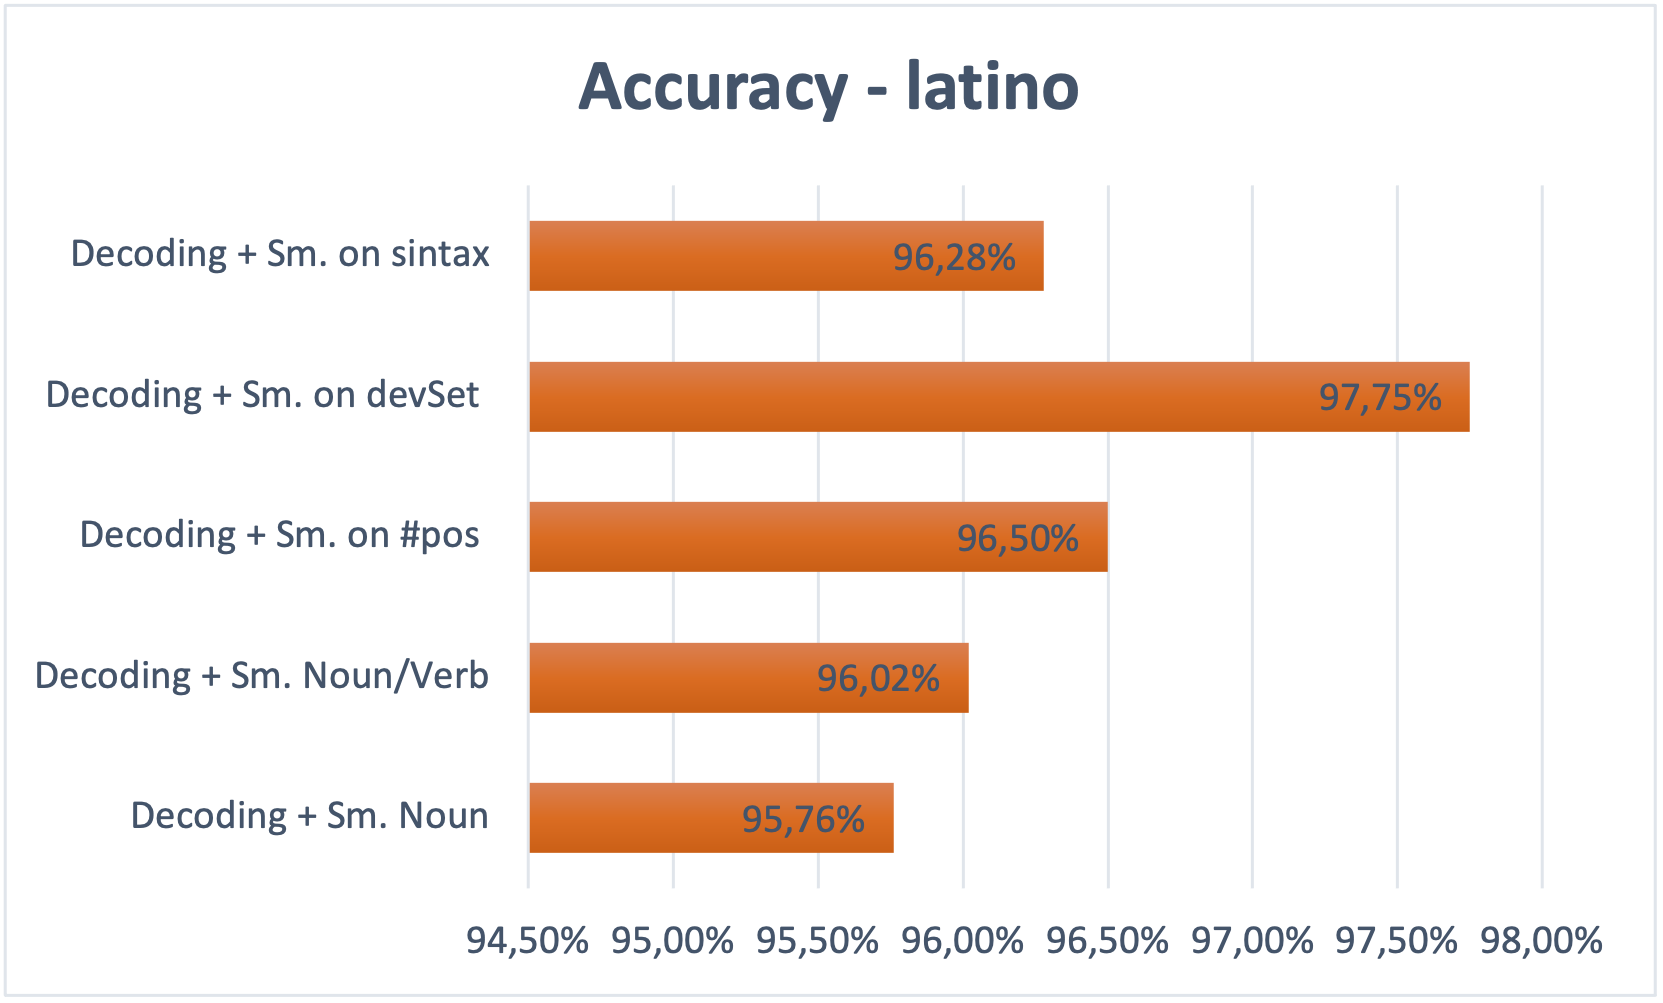
\includegraphics[scale=0.5]{fig/AccuracyLatino.png}
   \caption{Score per il latino}\label{fig:scoreLatino}
\end{figure}

\begin{figure}[H]
   \centering
   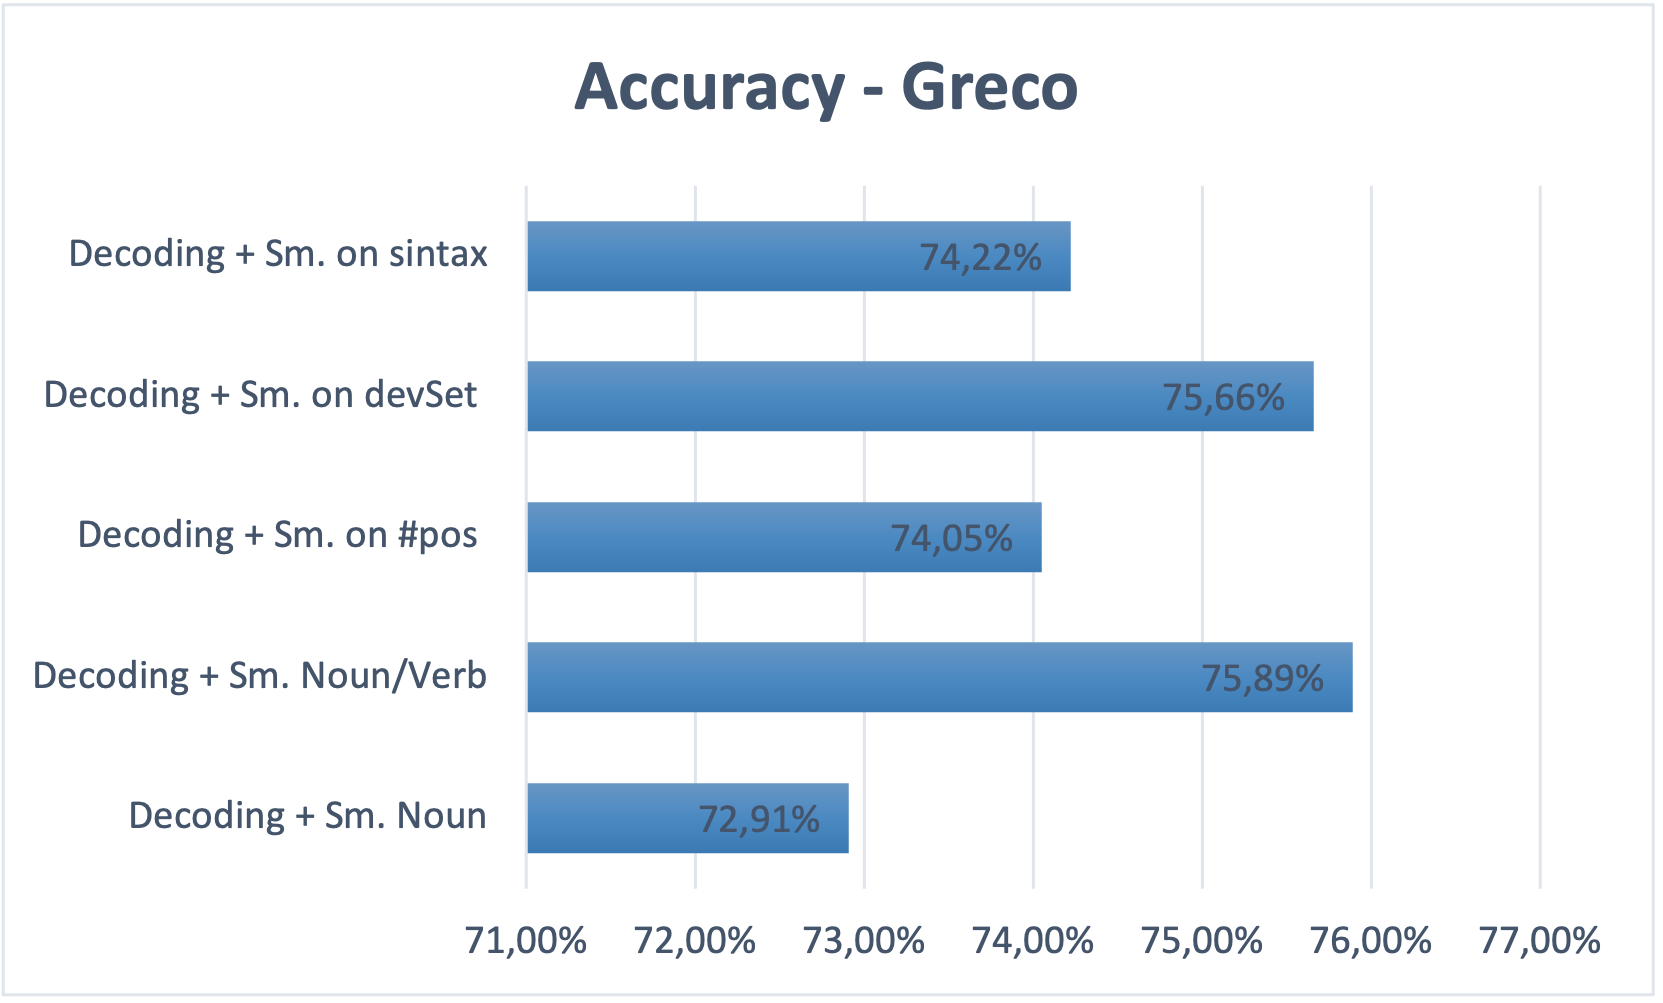
\includegraphics[scale=0.5]{fig/AccuracyGreco.png}
   \caption{Score per il greco}\label{fig:scoreGreco}
\end{figure}

Generalmente entrambe le lingue presentano analogie per quanto riguarda il testing applicando le diverse strategie di smoothing.
Infatti, la strategia di smoothing basata sui nomi è per entrambe la peggiore, contrariamente a quella basata sul development set che si comporta decisamente meglio.
Lo smoothing basato sulle regole sintattiche migliora leggermente lo score rispetto allo smoothing basato sui nomi, non riuscendo tuttavia a posizionarsi nella parte alta della classifica delle strategie.
\\
\\Accanto a questa analisi, poniamo di seguito quella dei tempi:

\begin{figure}[H]
   \centering
   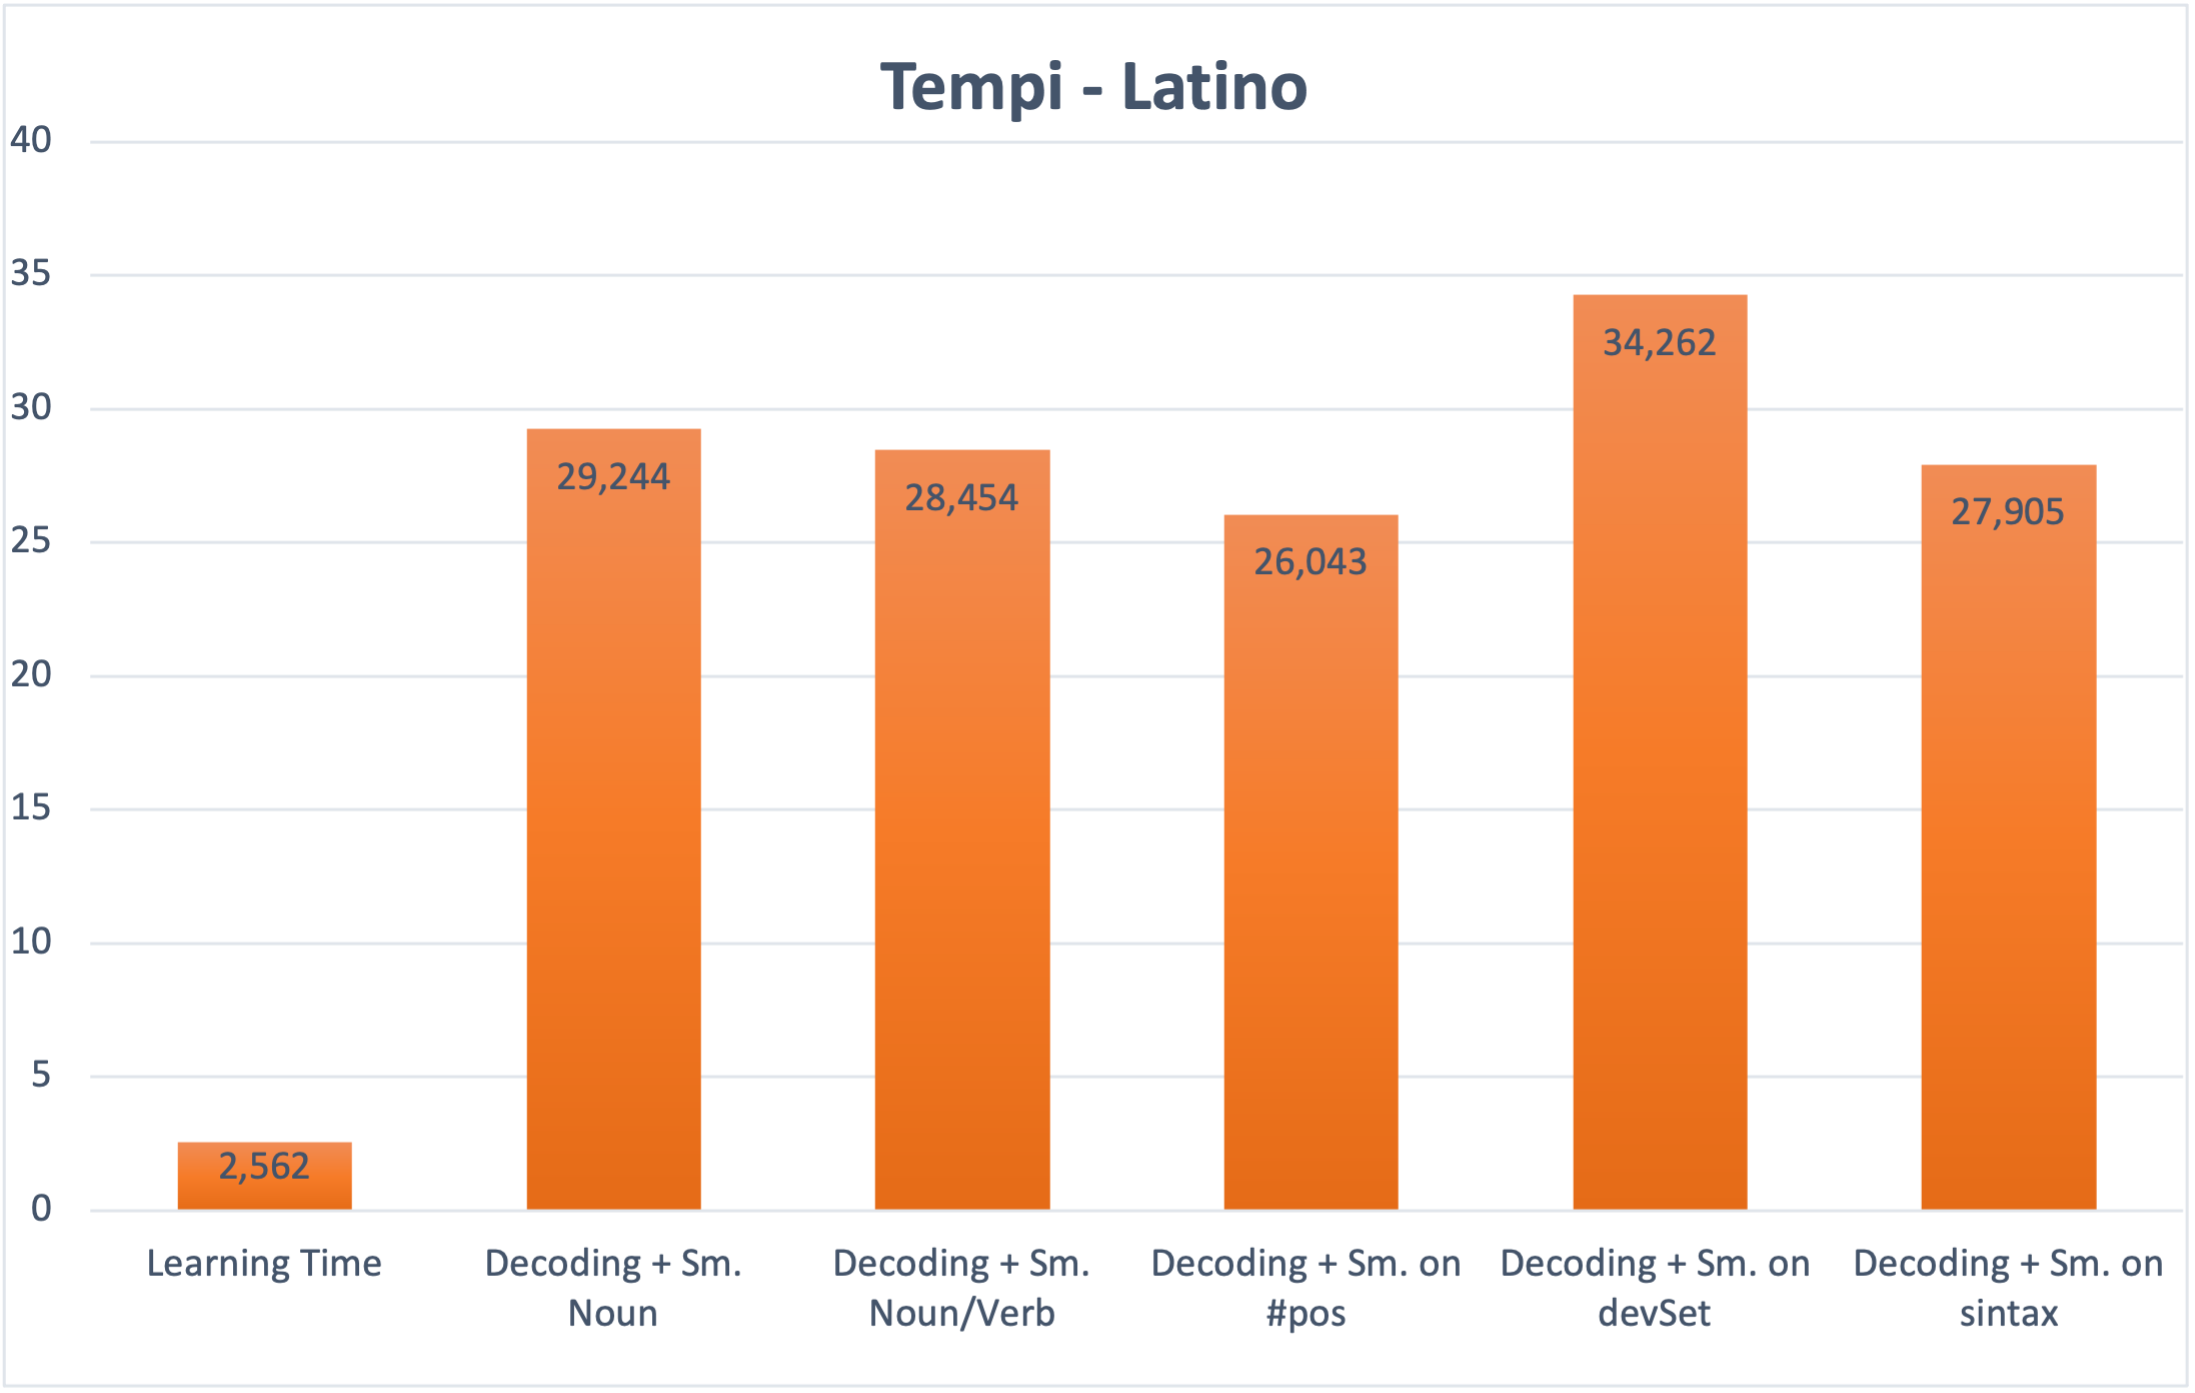
\includegraphics[scale=0.5]{fig/TempiLatino.png}
   \caption{Tempi in secondi per il latino}\label{fig:tempiLatino}
\end{figure}

\begin{figure}[H]
   \centering
   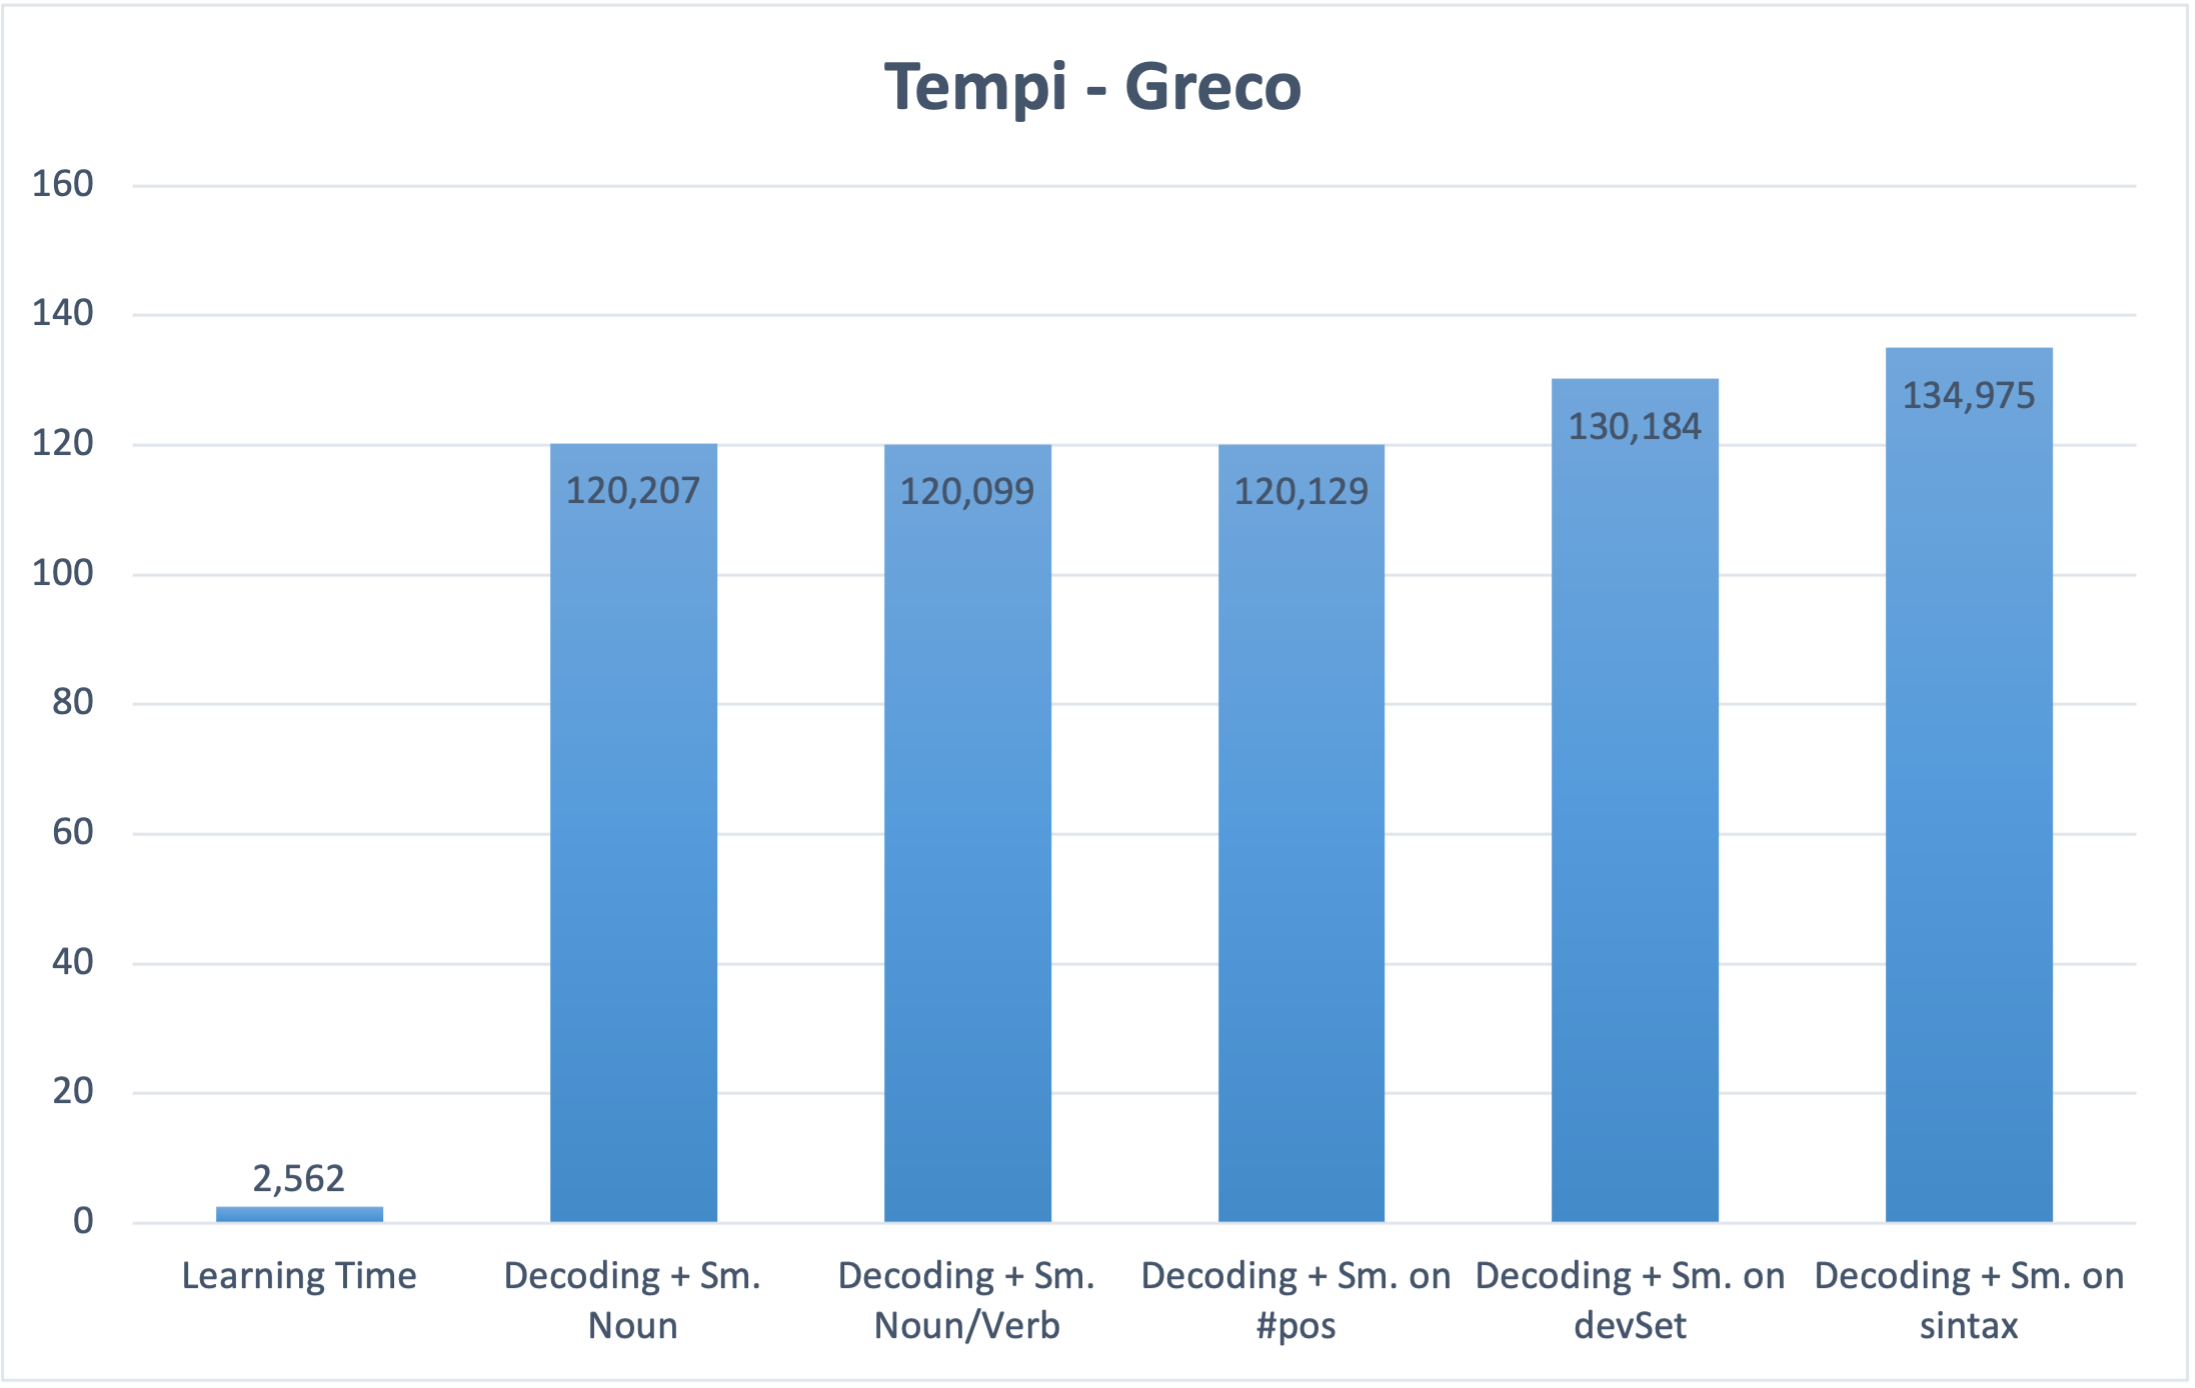
\includegraphics[scale=0.5]{fig/TempiGreco.png}
   \caption{Tempi in secondi per il greco}\label{fig:tempiGreco}
\end{figure}

Quello che risalta è la differenza in termini di ordine di grandezza fra le due lingue. La causa è dovuta probabilmente all’encoding che l’interprete Python ha dovuto effettuare per l’alfabeto greco. Ciononostante, per tutti i test con i vari smoothing il tempo di esecuzione è molto simile.
\\Come era prevedibile sia per il greco che per il latino i tempi di esecuzione minori sono per le strategie di smoothing che impiegano meno tempo ad essere calcolate: per entrambe infatti, la strategia basata sul development set è la più lenta.
\\
\\Per quanto riguarda gli errori più comuni commessi dal sistema: generalmente i tag che inducono maggiormente in errore sono per il latino i PROPN, i VERB e gli ADJ; invece, per il greco sono gli ADV, gli ADJ e i VERB. La motivazione è probabilmente dovuta alla natura delle termini: ad esempio i nomi propri sono molti e vari quindi, con poche occorrenze nel training corpus; mentre nel greco gli aggettivi neutri possono fungere da avverbi e condurre il sistema in errore.
%%%%%%%%%%%%%%%%%%%%%%%%%%%%%%%%%%%%%%%%%%%%%%%%%%%%%%%%%%%%%%%%%%%%
\section{Simple Baseline e confronto}
L’ultima parte dell’analisi dei dati ha previsto il confronto dei risultati con una semplice baseline. Ne è stata, quindi, implementata una con le seguenti caratteristiche:

\begin{itemize}
    \item nella fase di learning si esaminano le  parole del training set e si memorizzano i tag più frequenti per queste.
    \item nella fase di decoding si assegnano alle parole del test set i tag ritrovati nel passo precedente. Qualora ci siano termini sconosciuti sarà assegnato automaticamente il tag ‘NOUN’.
\end{itemize}

\begin{figure}[H]
   \centering
   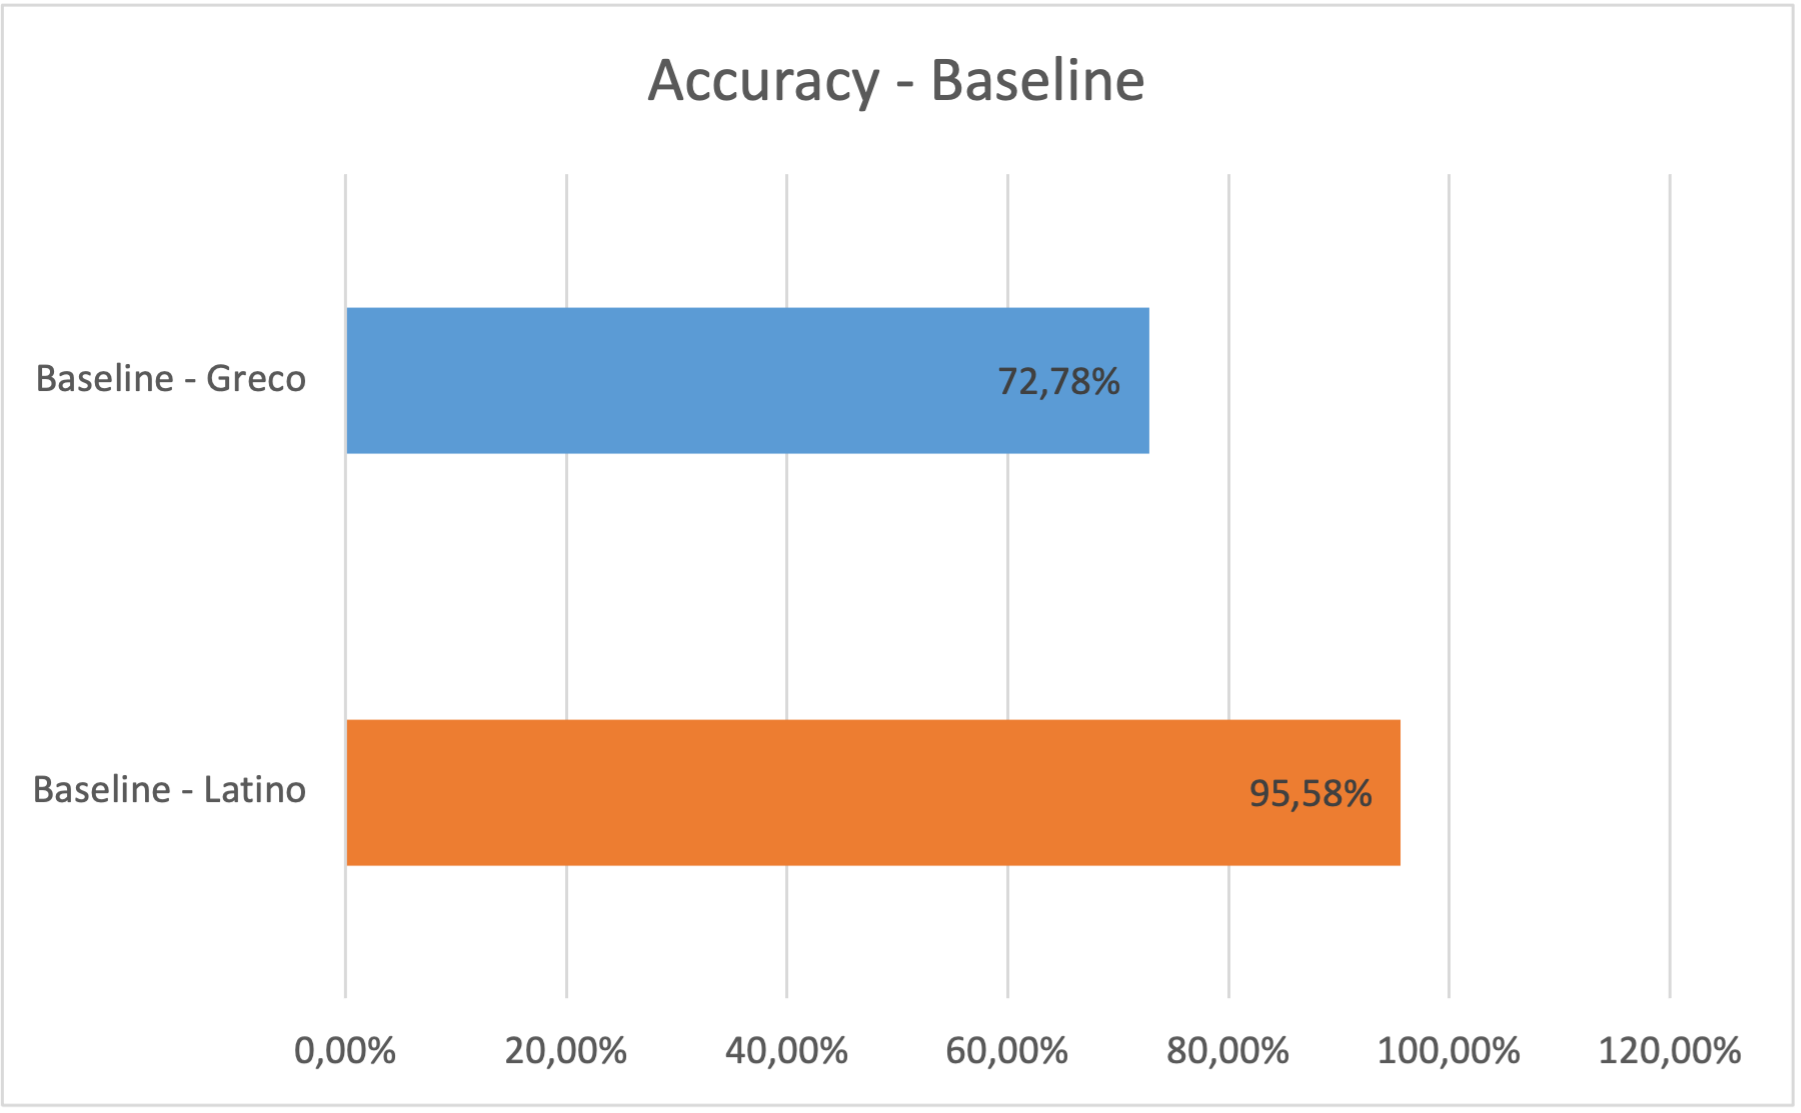
\includegraphics[scale=0.5]{fig/AccuracyBaseline.png}
   \caption{Score per la baseline - semplice}\label{fig:scoreBaselie}
\end{figure}

\begin{figure}[H]
   \centering
   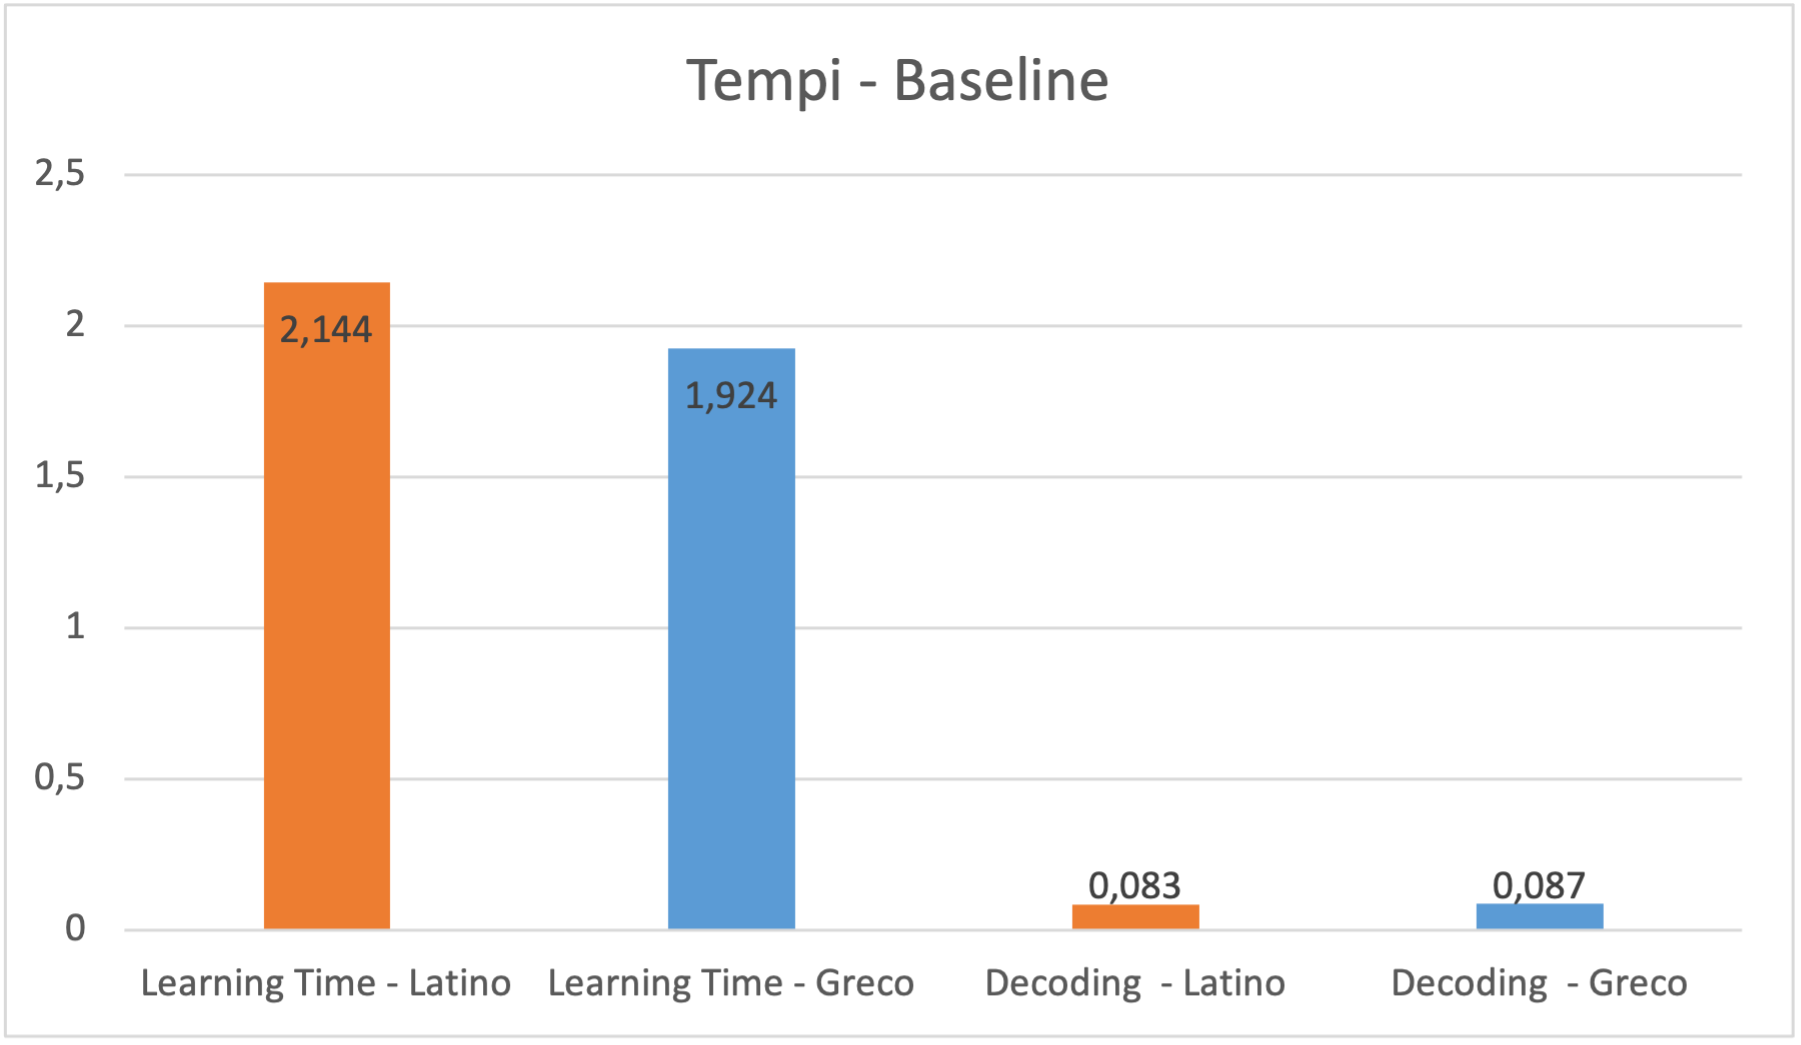
\includegraphics[scale=0.5]{fig/TempiBaseline.png}
   \caption{Tempi per la baseline - semplice}\label{fig:tempiBaselie}
\end{figure}

Da questi dati scaturisce una domanda nota in letteratura:  ‘Quanto è vantaggioso il compromesso tra tempo e accuratezza?’ 
\\Di fatti esaminando solo le percentuali di accuratezza  per la lingua latina si evince come la differenza tra questa e ad esempio quella implementata con la strategia di smoothing basata sui nomi è di circa due decimi. Tuttavia, il tempo necessario per computare i due risultati è notevolmente diverso: il sistema della simple baseline è ovviamente molto più veloce. Tali risultati sono ancora più enfatizzati per la lingua greca. 

Prima di giungere alle conclusioni, si può trarre un’analogia tra gli errori più comuni ritrovati in output e il sistema implementato. Anche in questo caso, quelli più comuni riguardano i tag elencati nella sezione precedente confermando l'ambiguità di questi.
\\
\\Il sistema implementato nel progetto è infine un buono strumento per effettuare PoS tagging. Le percentuali di accuratezza per ogni strategia di smoothing sono maggiori di quella di una semplice baseline e questi si avvicinano ai punteggi umani. Tuttavia, in base al task richiesto e alla capacità di calcolo del sistema potrebbe essere meglio rivolgere lo sguardo verso sistemi più semplici che garantiscano risultati leggermente peggiori, ma con vantaggi significativi dal punto di vista computazionale. Un esempio è per lingue complesse come il greco dove la complessità temporale gioca un ruolo importante; al contrario è un’ottima soluzione usare il PoS tagger con smoothing basato su un development set qualora si disponga di corpus ricchi.\\

\textbf{Nota}: i risultati sono stati calcolati con una macchina con le seguenti specifiche hardware e software:
\begin{figure}[H]
    \centering
    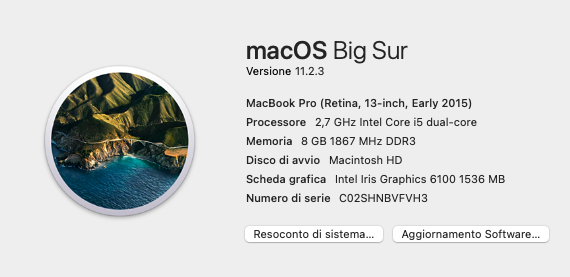
\includegraphics[scale=0.5]{fig/Sistema.png}
    \label{fig:sistema}
\end{figure}
%%%%%%%%%%%%%%%%%%%%%%%%%%%%%%%%%%%%%%%%%%%%%%%%%%%%%%%%%%%%%%%%%%%%
\newpage
\end{document}
